\documentclass[12pt,letterpaper]{article}
\usepackage{graphicx,textcomp}
\usepackage{natbib}
\usepackage{setspace}
\usepackage{fullpage}
\usepackage{color}
\usepackage[reqno]{amsmath}
\usepackage{amsthm}
\usepackage{fancyvrb}
\usepackage{amssymb,enumerate}
\usepackage[all]{xy}
\usepackage{endnotes}
\usepackage{lscape}
\newtheorem{com}{Comment}
\usepackage{float}
\usepackage{hyperref}
\newtheorem{lem} {Lemma}
\newtheorem{prop}{Proposition}
\newtheorem{thm}{Theorem}
\newtheorem{defn}{Definition}
\newtheorem{cor}{Corollary}
\newtheorem{obs}{Observation}
\usepackage[compact]{titlesec}
\usepackage{dcolumn}
\usepackage{tikz}
\usetikzlibrary{arrows}
\usepackage{multirow}
\usepackage{xcolor}
\newcolumntype{.}{D{.}{.}{-1}}
\newcolumntype{d}[1]{D{.}{.}{#1}}
\definecolor{light-gray}{gray}{0.65}
\usepackage{url}
\usepackage{listings}
\usepackage{color}

\definecolor{codegreen}{rgb}{0,0.6,0}
\definecolor{codegray}{rgb}{0.5,0.5,0.5}
\definecolor{codepurple}{rgb}{0.58,0,0.82}
\definecolor{backcolour}{rgb}{0.95,0.95,0.92}

\lstdefinestyle{mystyle}{
	backgroundcolor=\color{backcolour},   
	commentstyle=\color{codegreen},
	keywordstyle=\color{magenta},
	numberstyle=\tiny\color{codegray},
	stringstyle=\color{codepurple},
	basicstyle=\footnotesize,
	breakatwhitespace=false,         
	breaklines=true,                 
	captionpos=b,                    
	keepspaces=true,                 
	numbers=left,                    
	numbersep=5pt,                  
	showspaces=false,                
	showstringspaces=false,
	showtabs=false,                  
	tabsize=2
}
\lstset{style=mystyle}
\newcommand{\Sref}[1]{Section~\ref{#1}}
\newtheorem{hyp}{Hypothesis}

\title{Problem Set 1}
\date{Due: January 28, 2026}
\author{Data Visualisation for Social Scientists}

\begin{document}
	\maketitle
	
	\section*{Instructions}
	\begin{itemize}
	\item Please show your work! You may lose points by simply writing in the answer. If the problem requires you to execute commands in \texttt{R}, please include the code you used to get your answers. Please also include the \texttt{.R} file that contains your code. If you are not sure if work needs to be shown for a particular problem, please ask.
\item Your homework should be submitted electronically on GitHub.
\item This problem set is due before 23:59 on Wednesday January 28, 2026. No late assignments will be accepted.
	\end{itemize}
	
	\vspace{1cm}
	\section*{Roll Call Votes in the European Parliament}

\subsection*{Data Manipulation}
First, you need to \href{https://personal.lse.ac.uk/hix/HixNouryRolandEPdata.HTM}{download data} from the first six elected European Parliaments on each MEP and how they voted in each recorded roll-call vote.
\vspace{.25cm}
	\lstinputlisting[language=R, firstline=1, lastline=11]{Vote.R} 
	\textit {I loaded both of the datasets into R}
\begin{enumerate}
\item Load these datasets into your global environment:
\begin{itemize}
	\item \texttt{mep\_info\_26Jul11.xls} (MEP characteristics, EP1–EP5)
	\item \texttt{rcv\_ep1.txt} (EP1 roll-call votes)
\end{itemize}

\item Briefly describe (2–3 sentences each) the unit of analysis and key variables in each of these two datasets.


\textit  {In the MEP dataset the unit of analysis is the MEP and the unit of analysis in the RCV dataset is a single MEP's vote in a roll call session. The key variables are: MEP's name, member state, national party, EP Group, and scores for the MEP dataset, For the RCV dataset the key variables are how the MEPs' voted and MEP name, MEP ID, member state, national party, and EP Group.}  

\item The \texttt{rcv\_ep1} data are in a wide format, with V1, V2, …, Vn as separate vote columns.
\begin{itemize}
	\item Identify which columns are ID/metadata (\textit{MEPID, MEPNAME, MS, NP, EPG}) and which columns are vote decisions ($V_1$…$V_n$). Tidy the voting data such that each row/observation is a single vote for a single MEP.
	\lstinputlisting[language=R, firstline=12, lastline=29]{Vote.R} 
	\textit {For this step, I needed to rename the column names for they are the same across the datasets. I also needed to rename the vote column to make sure they are clearly indicated as votes. In the next step I needed to pivot the data so that there is one row per MEP vote. Then I needed to convert the numeric codes for the votes into text.} 
	\item Create a summary table of counts of decision categories (e.g. Yes/No/Abstain/Present but did not vote/Absent) across all votes.
	\lstinputlisting[language=R, firstline=30, lastline=34]{Vote.R} 
	\begin{verbatim}
		VoteLabel                 Count
		<chr>                     <int>
		1 Present but did not vote 109224
		2 Not an MEP               103618
		3 Absent                    99753
		4 Yes                       88185
		5 No                        75171
		6 Abstain                    9577
	\end{verbatim}
\end{itemize}
\item  Construct a new dataset that combines MEP-level information with their vote decisions from EP1 in long format (from part 3). Check for missingness.
\lstinputlisting[language=R, firstline=35, lastline=53]{Vote.R}
\textit {In the first step, I extracted EP1 metadata from the Excel sheets to keep only the relevant columns for each MEP. I ensured that the MEPID column had the same type (character) in both the metadata and the voting dataset so they could be merged correctly. I then combined the vote data with the metadata using a left join and checked the resulting dataset for missing values}
\begin{verbatim}
	 A tibble: 1 × 12
	MEPID MEPNAME    MS    NP   EPG VoteNumber  Vote VoteLabel
	<int>   <int> <int> <int> <int>      <int> <int>     <int>
	1     0       0     0     0     0          0     0         0
	#  4 more variables: `National Party` <int>, `EP Group` <int>,
	#   `NOM-D1` <int>, `NOM-D2` <int>
		\end{verbatim} 
\item Compute, for each EP group in EP1:
\begin{itemize}
	\item The mean rate of Yes votes (Yes over Yes+No+Abstain) across all roll calls.
		\item The mean abstention rate.
	\item The mean vote preferences along the two contested dimensions (NOM-D1 and NOM-D2).
		\lstinputlisting[language=R, firstline=55, lastline=79]{Vote.R}
				\textit {In this step, I first filtered the combined EP1 dataset to include only valid votes, keeping rows where the VoteLabel was “Yes,” “No,” or “Abstain.” I then grouped these votes by European Parliament group (EPG) and calculated two measures of voting behavior for each group: the proportion of votes that were “Yes”  and the proportion of abstentions. Separately, I extracted the NOMINATE scores  for each MEP, removed any duplicate rows to ensure one row per MEP, converted the scores to numeric values, and computed the mean score on each dimension by EP group. Finally, I merged the vote statistics with the NOMINATE averages using a left join to produce a summary table  showing both voting cohesion and ideological position for each EP group. showing both voting cohesion and ideological position for each EP group.}

\end{itemize}{}
\end{enumerate}

\begin{verbatim}
	EPG   yes_rate abstention_rate mean_NOM_D1 mean_NOM_D2
	<chr>    <dbl>           <dbl>       <dbl>       <dbl>
	1 C        0.415          0.0752      0.811       0.530 
	2 E        0.509          0.0215      0.512      -0.277 
	3 G        0.512          0.0697      0.280      -0.818 
	4 L        0.486          0.0632      0.409      -0.324 
	5 M        0.528          0.0800     -0.357      -0.201 
	6 N        0.581          0.0562      0.250      -0.386 
	7 R        0.457          0.265      -0.586      -0.0419
	8 S        0.576          0.0574     -0.0980      0.261 
	> 		
\end{verbatim}
\subsection*{Data Visualization}

\begin{enumerate}
	\item Plot the distribution of the first NOMINATE dimension by EP group, and explain any trends you see.
	
	\lstinputlisting[language=R, firstline=82, lastline=101]{Vote.R} 
	\textit {This plot shows that voting behavior is associated with party affiliation. The same party groups tend to vote similarly. }
	\begin{center}
		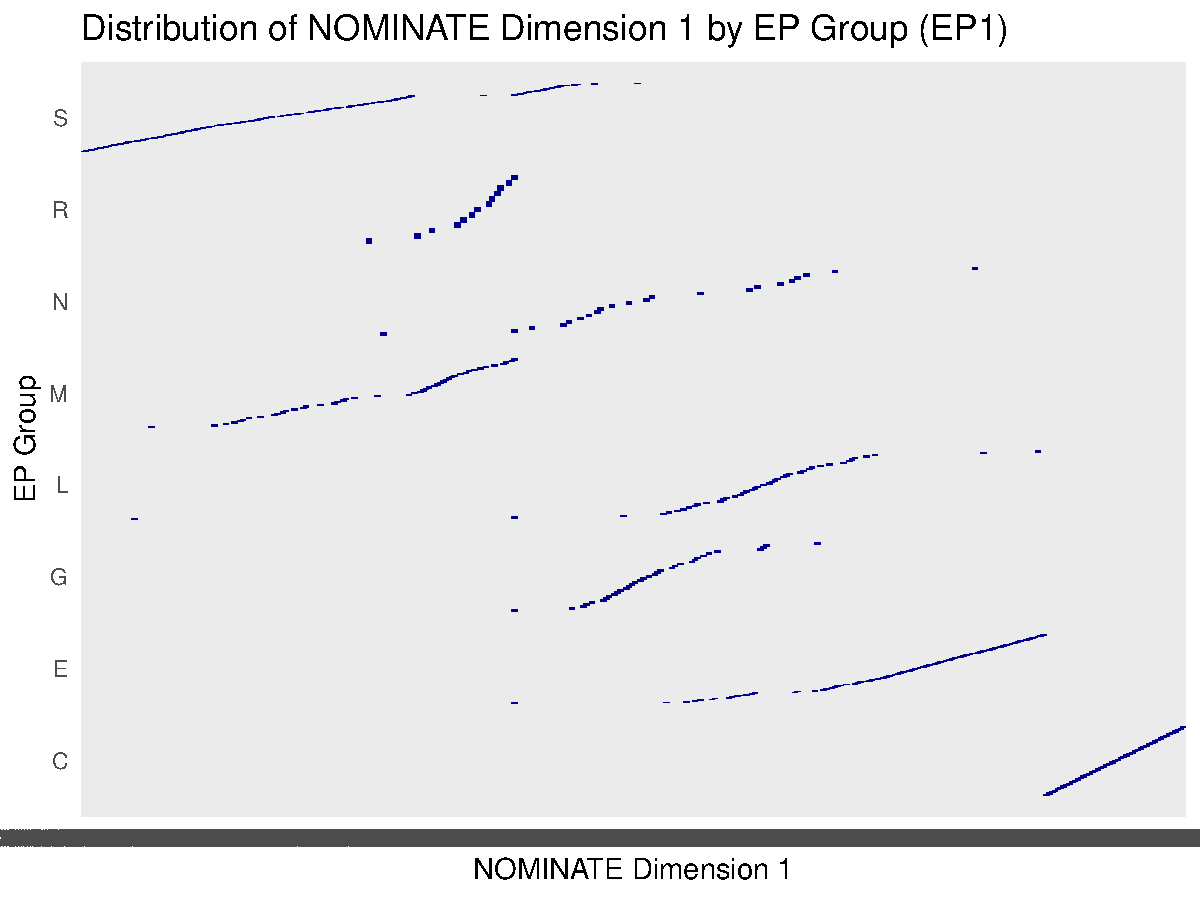
\includegraphics[width=0.7\textwidth]{vote_graph_one.pdf}
	\end{center}
	
	\item Make a scatterplot of \textit{nomdim1} (x-axis) and \textit{nomdim2} (y-axis), with one point per MEP and color by EP group.
	
		\lstinputlisting[language=R, firstline=103, lastline=128]{Vote.R} 
			\textit {In the scatterplot, MEPs from Group C and Group E cluster tightly, indicating that members of these groups are very aligned in their voting behavior. By contrast, Group S is more spread out across the NOMINATE dimensions, showing that its members are less cohesive and have more variation in their voting preferences. }
			\begin{center}
			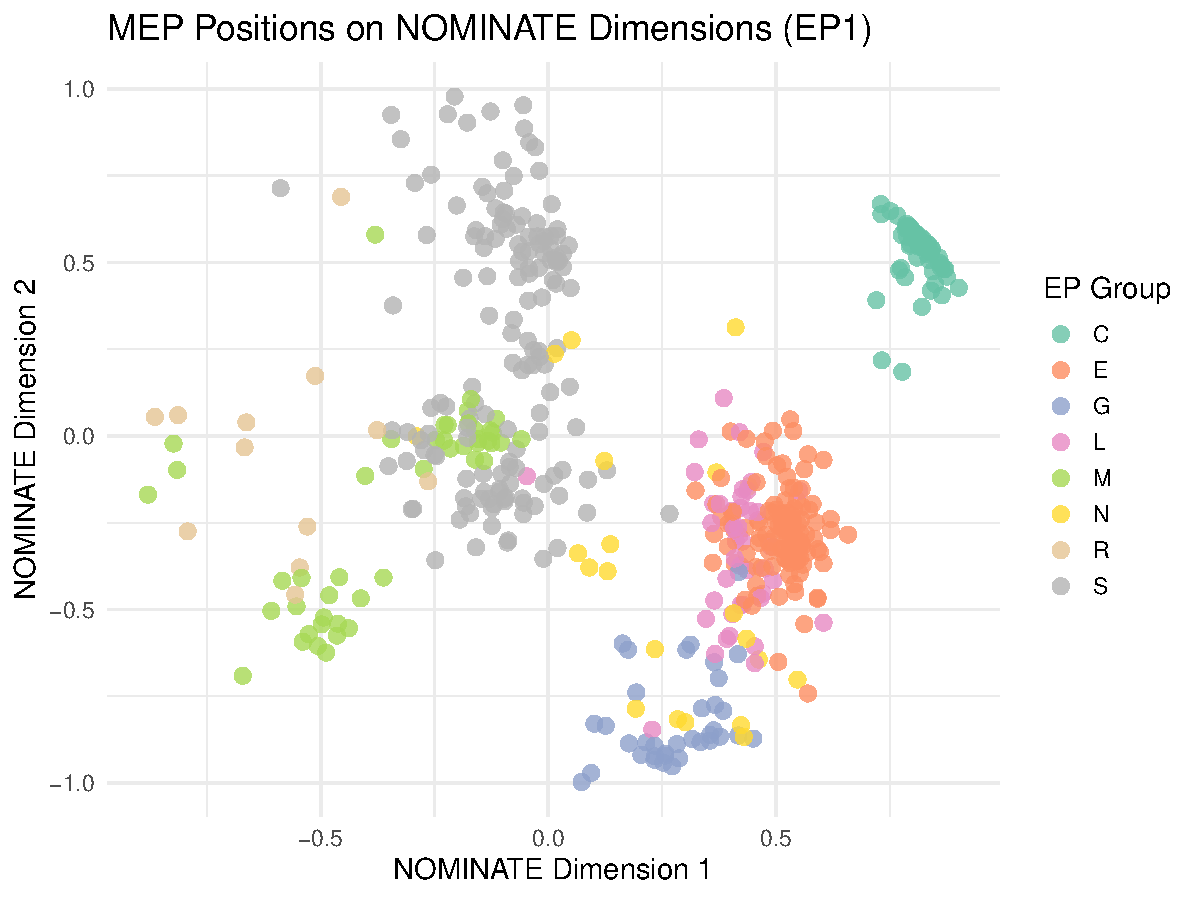
\includegraphics[width=0.7\textwidth]{vote_graph_two.pdf}
		\end{center}
	
	
	\item Produce a boxplot of the proportion voting \textit{Yes} by EP group to visualize cohesion.
	
	\lstinputlisting[language=R, firstline=130, lastline=156]{Vote.R} 
	
		\textit {The boxplot shows substantial differences in voting cohesion across EP groups. EP Group R exhibits the widest spread in the proportion of Yes votes, indicating considerable internal disagreement among its members. In contrast, EP Group C has the narrowest spread, suggesting a high level of internal cohesion and more disciplined voting behavior.}
			\begin{center}
		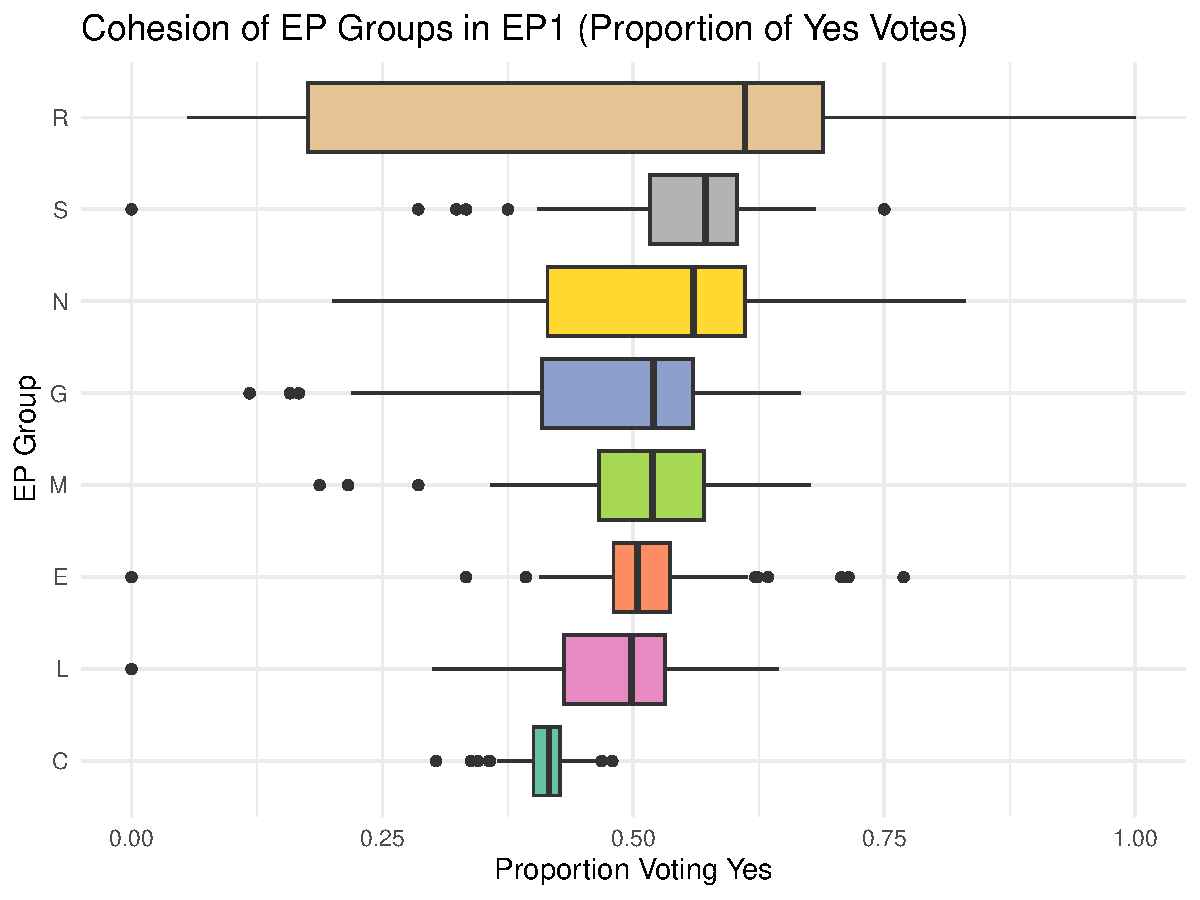
\includegraphics[width=0.7\textwidth]{vote_graph_three.pdf}
	\end{center}
	
	
	\item Display the proportion voting \textit{Yes} per year by national party using a bar plot.
	
		\lstinputlisting[language=R, firstline=158, lastline=193]{Vote.R} 
			\textit {This plot is showing that most parties voted yes above 40 percent but there was two parties that has very low yes votes. }
			\begin{center}
			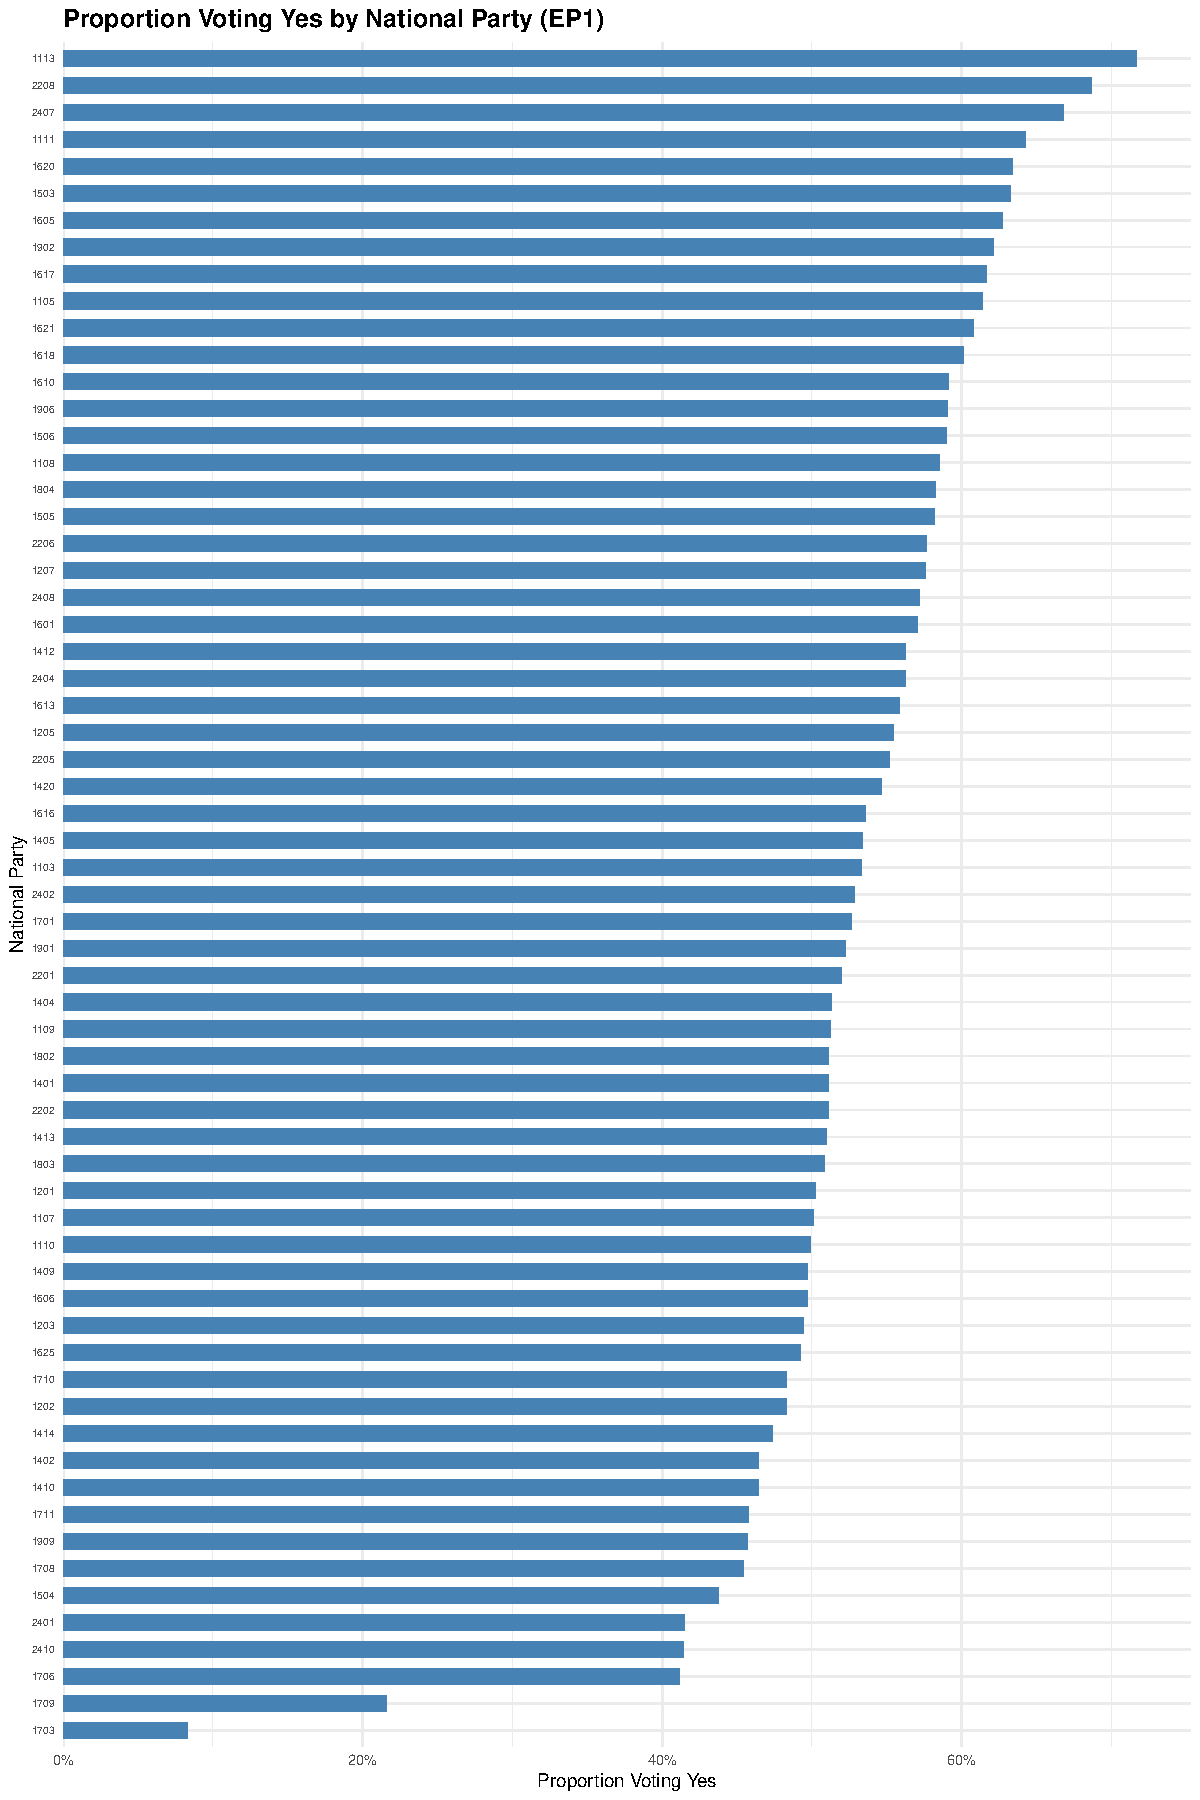
\includegraphics[width=0.7\textwidth]{vote_graph_four.pdf}
		\end{center}
		
	
	

\end{enumerate}


\end{document}
